\documentclass[12pt,a4paper]{article}
\usepackage[utf8]{inputenc}
\usepackage[german]{babel}
\usepackage[T1]{fontenc}
\usepackage{amsmath}
\usepackage{amsfonts}
\usepackage{amssymb}
\usepackage{graphicx}
\usepackage[left=2cm,right=2cm,top=2cm,bottom=2cm]{geometry}
\author{Tim}

\begin{document}

\tableofcontents
\newpage

\section{Schallgeschwindigkeit in Gasen}

\subsection{Resonanzfrequenzen in Röhre mit fester Länge}

\subsubsection{Versuchsbeschreibung}

Ziel des Versuchs ist die Erfassung der Frequenzabhängigkeit einer stehenden Welle bei fester Resonatorlänge am schallharten Abschluss.\\
In einem geschlossenen Rohr werden Schallwellen erzeugt, welche an den Rohrenden reflektiert werden. Durch die Überlagerung von einlaufenden und reflektierten Wellen kommt es zur Ausbildung von stehenden Wellen. Dabei gibt es Orte an denen der Schalldruck für alle Zeiten verschwindet (Knoten). Für diesen Versuch sind die Druckbäuche von Interesse, für welche die Druckamplitude maximal ist.\\
Bei fester Rohrlänge erhält man für die Resonanzfrequenzen, bei denen der Druck maximal ist den Zusammenhang:

\begin{equation}
	f_n=\frac{n\cdot v}{2L}
\end{equation}

mit der Rohrlänge $L$, der Ordnung der Resonanz $n$ der Schallgeschwindigkeit\footnote{Eigentlich Phasengeschwindigkeit, ohne Dispersion stimmt diese mit der Schallgeschwindigkeit überein.}  $v$ und der Frequenz $f_n$.
Misst man nun die Frequenz bei bekannter Länge L, so kann damit die Schallgeschwindigkeit bestimmt werden.\\

\subsubsection{Versuchsaufbau und Durchführung}

\begin{figure}
	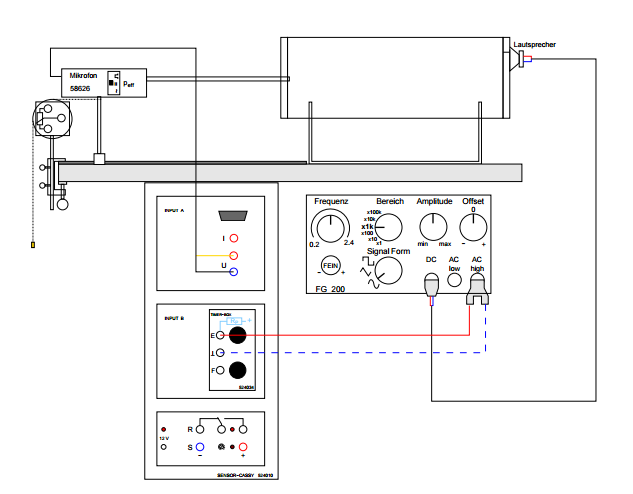
\includegraphics[width=\linewidth]{aufbau}
	\caption[Aufbau]{Schematischer Versuchsaufbau (Quelle: Praktikumsskript S.40)}
	\label{fig:aufbseite40}
\end{figure}
	


Die Röhre wird auf beiden Seiten verschlossen. An der einen Seite befindet sich ein Lautsprecher, auf der anderen das Mikrofon welches im Effektivwertmodus betrieben wird.
Mit dem BNC-Lemo-Adapter wird der Lautsprecher an den niederohmigen DC-Ausgang des Funktionsgenerators angeschlossen. Der rechte Hochpegel AC-Ausgang wird mittels der CASSY Timer-Box an den Kanal B des Sensor-CASSY angeschlossen. Das Mikrofon ist mit dem Kanal A des CASSY verbunden. Ein schematischer Aufbau findet sich in Abb.  \ref{fig:aufbseite40}.\\
Für den Funktionsgenerator wurden für die Signalform eine Sinusschwingung mit Offset null und mittiger Amplitude im Bereich $0.2-2.4 kHz$ gewählt.\\

Für den Kanal A des CASSY wurde der Messbereich der Spannung zu $0-3V$ gewählt mit Nullpunkt links und gemittelt über $1s$.
Die Timer-Box an Kanal B ist auf den Bereich bis $5000Hz$ mit Torzeit $1s$ eingestellt. Die Messung selbst wird manuell durchgeführt.\\

Zunächst wird die Länge des Rohres mit einem Maßband gemessen.
Die Frequenz des erzeugten Tons wird fortwährend erhöht und dabei manuell Spannungsmesswerte des Mikrofons aufgenommen. Die Lage der Resonanzfrequenzen kann bereits vorher abgeschätzt werden. Diese Bereiche werden mit dem Funktionsgenerator sehr kleinschrittig durchlaufen um die schmalen Resonanzen möglichst gut zu erfassen.

\subsubsection{Versuchsauswertung}
\begin{figure}
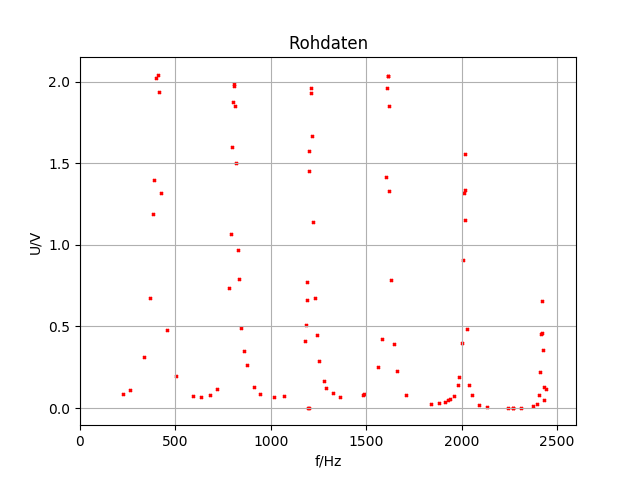
\includegraphics[width=\linewidth]{rohres}
\caption{Rohdaten der Resonanzmessung}
\label{fig:rohresonanz}
\end{figure}
Die Länge wurde mit einem Maßband der Güteklasse II zu $L=42.8cm$ gemessen. Der statistische Ablesefehler beträgt $\sigma_{L,stat.}=0.3mm$, der systematische Fehler ergibt sich zu $\sigma_{L,syst.}=0.7mm$.

Zur Bestimmung der Frequenzpeaks wurde der gesamte Messbereich symmetrisch um die erste Abschätzung der Peaks in je sechs Intervalle mit einer Gesamtlänge von $240Hz$ ($f_n \pm 120Hz$) unterteilt. Diese Intervalle wurden in $10Hz$ Schritten zehnmal verkleinert, einmal mit festgehaltenem linken Rand, einmal mit festgehaltenem rechten Rand und einmal mit Verkleinerung beider Ränder. Dabei wurde jedes mal mittels der peak-Funktion der Praktikumsbibliothek die Position der Peaks bestimmt. Aus den so entstehenden 33 Werten für jede Resonanzfrequenz wurde Mittelwert und Standardabweichung gebildet. Damit ergeben sich dann die Resonanzfrequenzen die Werte in Tab. \ref{resonanztabelle}.\\

\begin{table}
\begin{center}

\begin{tabular}{|c|c|c|}

\hline 
$n$ & $f_n$[Hz] & $\sigma_{f_n}$[Hz] \\ 
\hline 
1 & 404,11 & 1.47 \\ 
\hline 
2 & 809,60 &  1.72 \\ 
\hline 
3 & 1209.22 & 1.29 \\ 
\hline 
4 & 1613.86 & 1.32 \\ 
\hline 
5 &   2013.32 & 1.29 \\ 
\hline 
6 & 2420.10 &     0.96 \\ 
\hline
\end{tabular}
\caption{Resonanzfrequenzen und Unsicherheiten}
\label{resonanztabelle}
\end{center}
\end{table} 

Eine lineare Regression ($f(n)=a \cdot n+b$) ergibt $a=402.94 Hz$, $\sigma_a=0.30 Hz$, $\b=1.40 Hz$ und $\sigma_b=1.32 Hz$. Eine grafische Darstellung des Ergebnisses findet sich in Abb. \ref{fig:resonanzregression}.  Bei sechs Datenpunkten und zwei zu bestimmenden Parametern erhält man für diese Anpassung $\chi^2/ndof=2.13$, was dafür spricht, dass mit obigem Vorgehen die Fehler etwas zu klein geschätzt wurden.\\

\begin{figure}
	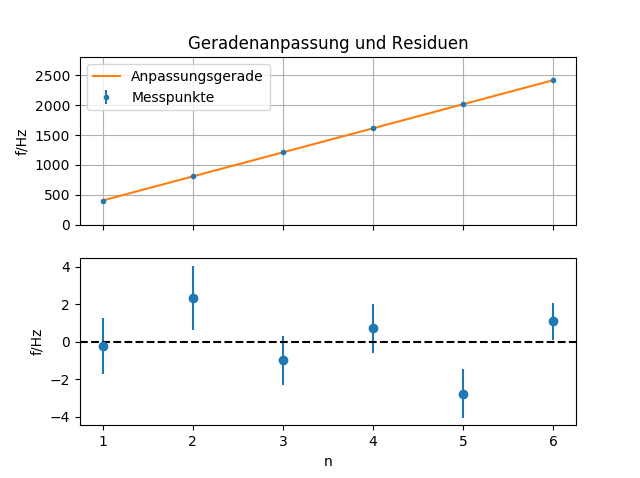
\includegraphics[width=\linewidth]{fitplot}
	\caption[Auswertung Resonanz]{Messpunkte und Regressionsgerade (oben) und
	Residuen (unten).}
	\label{fig:resonanzregression}
\end{figure}


Aus $a=\frac{v}{2L}$ (vgl. oben) erhält man:
\begin{equation}
	v=2La=344.91 m/s
\end{equation}

Für den statistischen Fehler erhält man mittels Fehlerfortpflanzung:
\begin{equation}
	\sigma_{v,stat.}=v \cdot \sqrt{(\frac{\sigma_a}{a})^2+		(\frac{\sigma_{L,stat.}}{L})^2}=0.35 m/s
\end{equation}

Der systematische Fehler ergibt sich durch Fortpflanzung des systematischen Fehlers des Maßbands.
\begin{equation}
	\sigma_{v,syst.}=\sqrt{4a^2 \cdot \sigma_{L,syst.}^2}		=2a \sigma_{L,syst.}=0.56 m/s
\end{equation}

Also insgesamt:
\begin{equation}
v=(344.91 \pm 0.35(stat.) \pm 0.56(syst.))m/s
\end{equation}

Eine Temperaturmessung unmittelbar vor Versuchsbeginn lieferte $T=24.4 C$. Die theoretisch vorhergesagte Schallgeschwindigkeit ist damit gegeben durch:
\begin{equation}
v=v_0 \sqrt{T/T_0} \quad \text{mit} \quad v_0=\sqrt{\frac{R \cdot \kappa T_0}			{M_{mol}}}
\qquad
\Rightarrow v=346.23 m/s
\end{equation}

Theoretischer und gemessener Wert liegen somit in guter Übereinstimmung weniger als zwei Standardabweichungen auseinander.




\subsection{Druckknoten einer stehenden Welle}

\subsubsection{Versuchsbeschreibung}
Ziel des Versuchs ist die Messung des Schalldruckprofils einer stehenden Welle bei fester Resonatorlänge.\\
Für diesen Versuch macht man sich nutze, dass die Positionen der Drucknoten der stehenden Schallwellen aufgetragen über $n$ auf einer Geraden mit Steigung  $\lambda/2$ liegen.

\subsubsection{Versuchsaufbau und Durchführung}
Zunächst wird am Frequenzgenerator die höchste Resonanzfrequenz (hier etwa $2017Hz$)\footnote{aus CASSY-Schwerpunktbestimmung} des vorherigen Teilversuchs eingestellt.
Der Aufbau des eigentlichen Versuchs ist größtenteils identisch mit Teilversuch eins. Anstelle des Piezo Hochtöners verwendet man hier ebenfalls den Kleinlautsprecher und am Kanal A des CASSY wird keine Timer-Box verwendet und direkt die Spannung gemessen. Der Messbereich der Spannung ist wieder $0-3V$ mit Nullpunkt links und gemittelt über $100ms$.\\
Der Widerstand am Kanal B wird im Bereich $0-3k \Omega $ gemessen.
Der Messparameter wird auf automatisch gestellt bei einer Intervalllänge von $100ms$.\\
Für Aufzeichnung des Druckverlaufs wird das zunächst am Rohrabschluss  befindliche Messende des Mikrofons möglichst gleichmäßig mit nicht mehr als $1cm/s$ vollständig in das Rohr hineingeschoben.

\subsubsection{Versuchsauswertung}

\begin{figure}
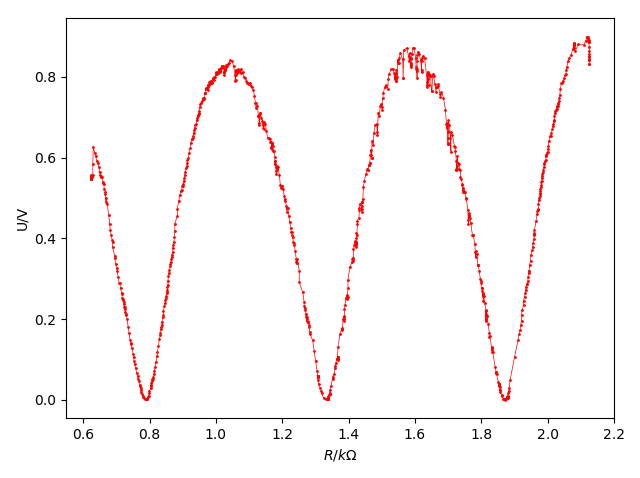
\includegraphics[width=\linewidth]{druckverlauf}
\caption{Druckverlauf innerhalb Rohres. Zu beachten ist das die Kurve von rechts ausgehend aufgezeichnet wurde.}
\label{Druckverlauf}
\end{figure}

Der Versuch die Knoten oder Bäuche (Minima bzw. Maxima in Abb. \ref{Druckverlauf}) mithilfe entsprechender Python-Funktionen zu bestimmen lieferte keine zufriedenstellende Ergebnisse.
Da zumindest die Minima sehr scharf abgebildet wurden ist die Bestimmung der Knoten grafisch vorgenommen worden (vgl. Tab.\ref{tab:Druckknoten}). Als Fehler auf die Bestimmung ist der Fehler auf die Widerstandsmessung verwendet worden.

\begin{table}
\begin{center}
\begin{tabular}{|c|c|c|}
\hline 
n & $R[k\Omega]$ & $\sigma[k\Omega]$ \\ 
\hline 
1 & 0.788  & 0.006 \\ 
\hline 
2 & 1.344  & 0.006 \\ 
\hline 
3 & 1.872 & 0.006 \\ 
\hline 
\end{tabular}
\caption[Druckknoten]{Knoten des Druckverlaufs}
\label{tab:Druckknoten}
\end{center}
\end{table}

Eine lineare Regression ($R(n)=a \cdot n+b$) ergibt $a=0.542k\Omega$, $\sigma_{a}=0.004k\Omega$, $b=0.251k\Omega$ und $\sigma_b=0.009k\Omega$. Eine grafische Darstellung findet sich in Abb. \ref{fig:Regression Druckverlauf}.\\
Für diese Anpassung erhält man $\chi^2/ndof=3.630$. Das spricht dafür das der Fehler auf die Knotenbestimmung zu gering abgeschätzt wurde.

\begin{figure}
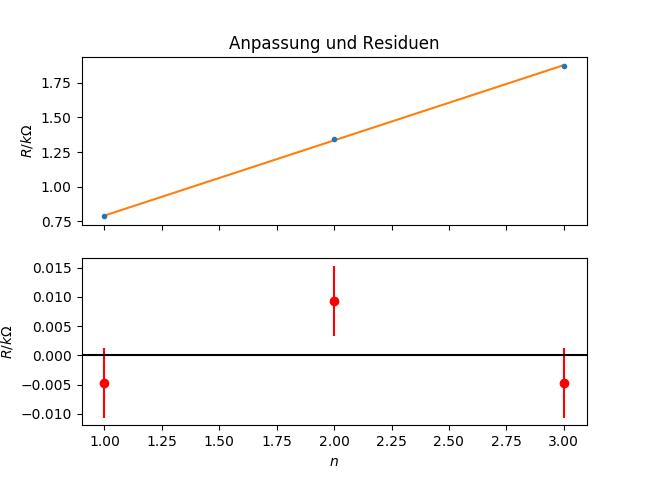
\includegraphics[width=\linewidth]{fitdruckknoten}
\caption[Regression Knoten]{Regressionsergebnis (oben) und Residuen (unten)}
\label{fig:Regression Druckverlauf}
\end{figure}

Mit der Steigung der Regression und dem Kalibrierungsfaktor $K=15.97 cm/k\Omega$ des Potentiometers ergibt sich für die Wellenlänge:
\begin{equation}
\lambda=2Ka=17.31cm
\end{equation}
Mit der eingestellten Frequenz von $f=2017.0Hz$ erhält man für die Schallgeschwindigkeit:
\begin{equation}
v=f \lambda = 349.14m/s
\end{equation}

Für die Frequenz wird ein Digitalisierungsfehler von $\sigma_f=0.3Hz$ angenommen($f$ gleichverteilt zwischen $2016.5-2017.5$). Der Fehler auf die Wellenlänge ist damit gegeben durch:
\begin{equation}
\sigma_{\lambda}=2K \sigma_a=0.13cm
\end{equation}
Für den statistischen Fehler der Schallgeschwindigkeit folgt dementsprechend:
\begin{equation}
\sigma_{v,stat.}=v \cdot \sqrt{(\frac{\sigma_{\lambda}}{\lambda})^2+(\frac{\sigma_f}{f})^2}=2.63m/s
\end{equation}

Der systematische Fehler ist durch den Fehler auf die Kalibrierung bedingt. Man erhält mit $\sigma_K=0.07cm/k\Omega$:
\begin{equation}
\sigma_{\lambda,syst.}=2a \sigma_K=0.08cm \quad \Rightarrow \quad \sigma_{v,syst.}=f \sigma_{\lambda,syst.}=1.61m/s
\end{equation}

Insgesamt ergibt sich damit:
\begin{equation}
v=(349.14 \pm 2.63(stat.) \pm 1.61(syst.))m/s
\end{equation}

Dem gegenüber steht der theoretische Wert mit $v_{Theorie}=346.23m/s$. Der gemessene Wert stimmt aufgrund der relativ großen Unsicherheiten relativ gut mit diesem überein.







\end{document}
